\def\mya{\theta-\theta(x)}

Consider the LINUX loss function defined by 
\[
  L(\mya) = e^{c(\mya)} - c(\mya) - 1.
\]
(a) Show that $L(\mya \ge 0 $ and plot this as a function of $(\mya)$ when $c= .1, .5, 1, 2$.\\
(b) Find $\hat\theta(x)$ the estimator that minimizes the Bayesian expected posterior loss.\\
(c) Find $\hat\theta(x)$ when $x_1,...x_n~|~\theta \sim N(\theta,1), \theta \sim N(\mu,\tau^2)$.

\subsection*{Solution:}
\subsubsection*{(a)}
Let $a = \mya$, then $L(\mya) = L(a) = e^a - a - 1$. 
\begin{align*}
  \ds\frac{d}{d a} L(a) &:= 0 \\
  e^a - 1 &= 0 \\
  a &= \ln(1) \\
  a &= 0 \\
\end{align*}

\noindent
So, $L(a)$ reaches a local extrema at $a=0 \Rightarrow L(a) = e^0 - 0 - 1 = 0$. 
That is, there is a local extrema at $(0,0)$.
And since $L''(a) = e^a > 0$, $(0,0)$ is a local minimum.\\

\noindent
Therefore, $L(\mya) \geq 0$.

\beginmyfig
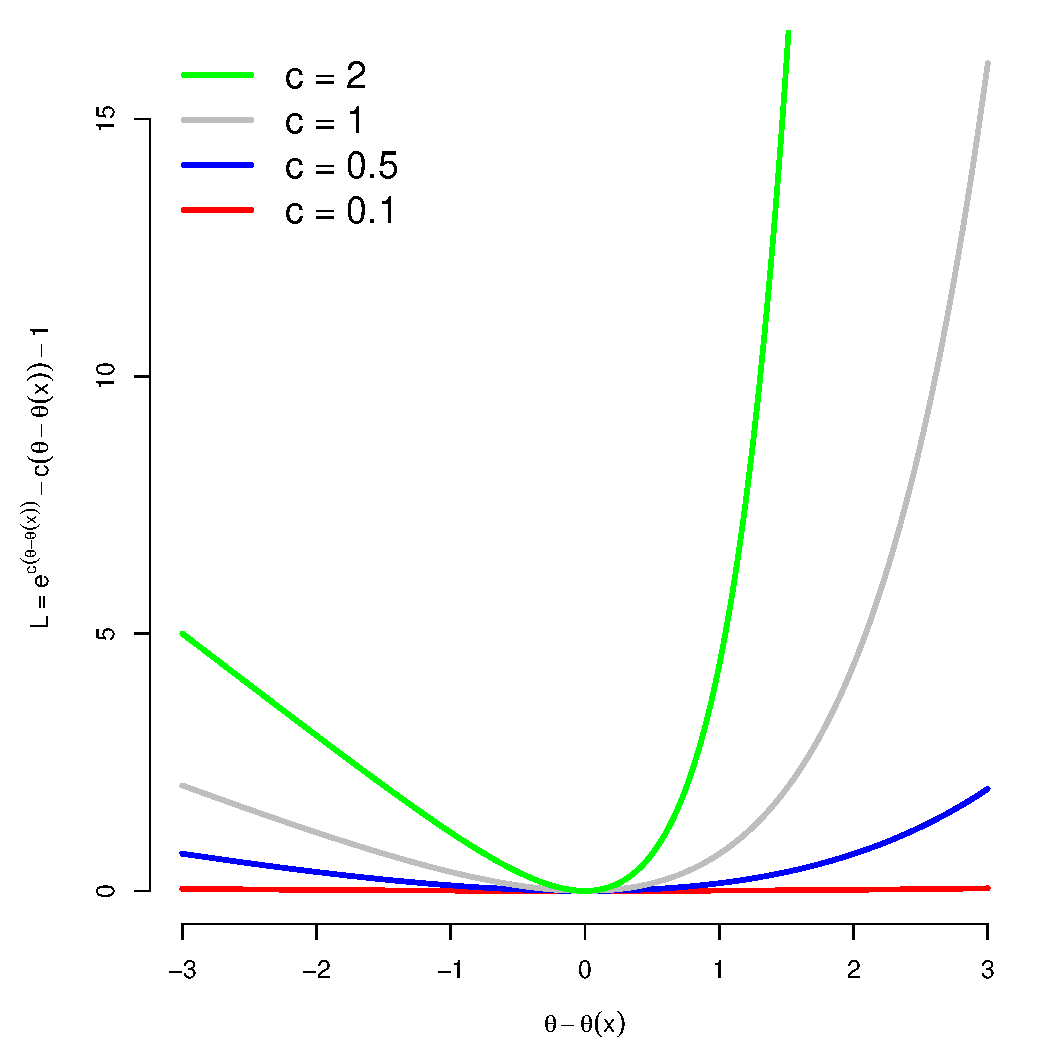
\includegraphics[scale=.7]{../img/fig1.pdf}
\caption{Plot for 7(a)}
\endmyfig
